\pagenumbering{gobble}
	\underline{\textbf{Implementation, integration and test plan}}\\\\
In section 2.2 of this document there is the desctiption of the components in which the whole system can be divided to split roles and functionalities and to simplify the development and the following testing.
As it is evident from the Component Diagram, the components can be classified into the following subsystems:
	\begin{itemize}
	\item Mobile client, made up by:
		\begin{itemize}
		\item Components: Mobile controller,  Data retriever, Health checker, Presentation mobile;
		\item Interfaces for external services: Map service interface, OS Bluetooth interface, Smartwatch interface, OS call service interface.
		\end{itemize}
	\item Web client;
	\item Business logic, made up by:
		\begin{itemize}
		\item Components: Individual controller, Third party controller, Authentication controller, Track4Run Individual controller, Track4Run Third party controller, Anonymous request builder, Storage controller;
		\item Interfaces for external services: Map service interface.
		\end{itemize}
	\item External components: Map service, OS Bluetooth service, OS call service, Smartwatch service, DBMS.\\
	\end{itemize}

A bottom-up strategy will be used to implement, integrate and test the system. Then the following steps will be performed:
	\begin{enumerate} 
	\item each subsystem will be implemented, integrated and tested;
	\item the subsystems will be integrated and tested togheter.\\
	\end{enumerate}
Since we cannot directly manage external components, we assume they are reliable and we use the provided interfaces to test our system.\\

To keep the integration and testing process more clear we can split the Business logic subsystem into the following subsystems:
	\begin{itemize}
	\item Individual subsystem: Individual controller and Storage controller;
	\item Authentication subsystem: Authentication controller and Storage controller;
	\item Thin third party subsystem: Third party controller and Storage controller;
	\item Full third party subsystem: Third party conroller, Anonymous request builder and Storage controller;
	\item Track4Run individual subsystem: Track4Run individual controller and Storage controller;
	\item Track4Run third party subsystem: Track4Run third party controller and Storage controller.\\
	\end{itemize}

To reach the same goal, in the Mobile client subsystem we can distinguish:
	\begin{itemize}
	\item Data4Help subsystem: Data retriever and Health checker;
	\item Transfer data subsystem: Data retriever and Mobile controller.\\
	\end{itemize}

Focusing the attention on the Mobile client, after having implemented and tested all the subsystems (step 1), it is needed to test the integration of all of them. Let's call the result Mobile client subsystem.
	\begin{figure}[H]
	\centering
	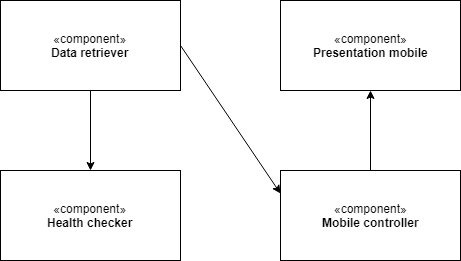
\includegraphics[scale=0.5] {images/integration/mobileClient.png}
	\caption {Mobile client subsystem}
	\end{figure}
	
Coming to the server side, after having implemented and tested all the subsystems, it is needed to test the integration of each of them with the Mobile client subsystem and with the Web client component.
More in detail:
	\begin{itemize}
	\item Mobile client subsystem and Individual subsystem;
	\item Mobile client subsystem and Authentication subsystem;
	\item Mobile client subsystem and Track4Run individual subsystem;
	\item Web client component and Authentication subsystem;
	\item Web client component and Full third party subsystem;
	\item Web client component and Track4Run third party subsystem.
	\end{itemize}
	
	\begin{figure}[H]
	\centering
	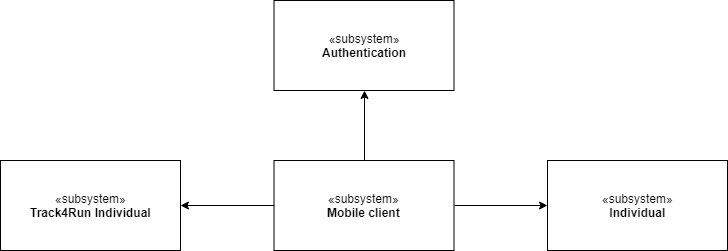
\includegraphics[scale=0.5] {images/integration/mobileAndServices.png}
	\caption {Mobile client tested with the other subsystems}
	\end{figure}
	
	\begin{figure}[H]
	\centering
	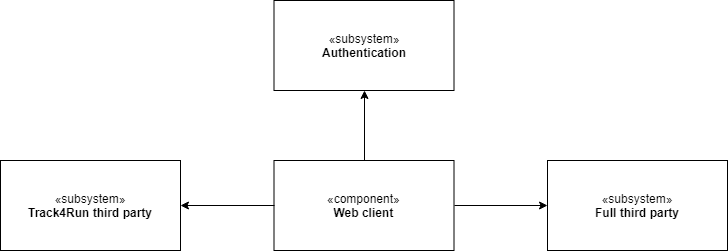
\includegraphics[scale=0.5] {images/integration/webAndServices.png}
	\caption {Web client tested with the other subsystems}
	\end{figure}
	
	After all the previous tests, a full integration test can be performed.
	
	\begin{figure}[H]
	\centering
	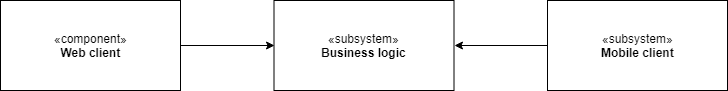
\includegraphics[scale=0.5] {images/integration/general.png}
	\caption {Test of the whole system}
	\end{figure}
	